\chapter{Search Algorithm and Neural Network Accelerated Indexing}

In this chapter, we define our problem and present our proposed solution.

\noindent{\bf Problem statement:} We want to extend keyword search to relational data using full-text index with the help of an embeddable neural network that optimizes the query processing pipeline. 
Given a relational database consists of $K$ relations $R_1, R_2, R_3, \dots, R_K$, the goal is to build a system that takes a partial tuple as user query and can find an optimally matching complete tuple $\vec r \in R_i$ ($i \in \{1, 2, \dots, K\}$) efficiently.

\section{Problem definition of partial tuple search}
In this section, we provide some definitions related to partial tuple search.
Let $R$ be a relational table.  Recall that $\Attr(R)$ is the attributes of $R$, and tuples in $R$ are mappings from $\Attr(R)$ to $\Values$.

\begin{definition}[Labeled values and partial tuple]
Let $R$ be a relational table.  A labeled value in $R$ is a pair $(l:x)$ where 
$l\in\Attr(R)\cup\{?\}$ and $x\in\Values$.  A partial tuple $\vec{x}$ is a set of labeled values: $\vec x = \{(l_i, x_i): i\in I\}$.  We define the attributes of a partial tuple $\vec x$ as the labels of the partial tuple:
$$\Attr(\vec x) = \{l_i\}_{i\in I}$$.
A partial tuple is considered {\bf\em complete} if $\Attr(\vec x) = \Attr(R)$.
\end{definition}

We will write $\vec x[l_i]$ to denote the corresponding value $x_i$.

Note that a partial tuple is a set of values and their respective attribute names from a relational table.  However, we allow a special symbol ``$?$" to be in place of the attribute name.  The special attribute ``$?$" indicates that the attribute name is unspecified (or unknown). The following example illustrates two partial tuples. The second partial tuple has a wild card ``?" as its attribute name:

\begin{example}
\begin{eqnarray*}
\vec s_1 &=& \{\mathrm{name}:\mathrm{Einstein}\} \\
\vec s_2 &=& \{\mathrm{name}:\mathrm{Einstein},\ \mathrm{?}: \mathrm{Professor}\}
\end{eqnarray*}
\end{example}

A query is a partial tuple: $\vec Q = \{(l_i, q_i): i\in I_Q\}$.  The values $q_i$ are keyword queries.
We want to find a complete tuple $\vec r \in R$ that matches $\vec Q$ optimally.  This requires us to define how to compare the partial tuple $\vec Q$ with a complete tuple $\vec r$.  The guiding principle of comparing the two tuples is to match labeled values from $\vec Q$ with those from $\vec r$ according to the following:
\begin{itemize}
    \item Match the labels if they are not the wild card ``$?$".
    \item Match the values using a fuzzy string matching score.
    \item Optimize the sum of similarities between labeled values from $\vec Q$ and those from $\vec r$.
\end{itemize}
Towards this end, we define the following similarity measures:

\begin{definition}[Similarity of labeled values]
\label{def:sim-labeled-values}

Consider two labeled values: $(l_1: x_1)$ and $(l_2, x_2)$,
where $l_1$ and $l_2$ are two labels from $\Attr(R)\cup\{?\}$.  The similarity between the two labels $l_1$ and $l_2$ is given by:
    $$
    \Sim(l_1, l_2) = \left\{
    \begin{array}{cl}
    1 & \mathrm{if}\ l_1 = l_2\ \mathrm{and}\ l_1\not=?,\ l_2\not=? \\
    0 & \mathrm{if}\ l_1 \not= l_2 \ \mathrm{and}\ l_1\not=?,\ l_2\not=? \\
    0.5 & \mathrm{if}\ l_1 = ?\ \mathrm{or}\ l_2 = ?
    \end{array}
    \right.
    $$
    Thus, whenever $l_i$ is the wildcard `` $?$", the similarity is 0.5. Otherwise, it is determined by the equality comparison of the two labels.

The similarity between the two values $x_1$ and $x_2$ is based on string comparison.  We utilize
the Jaccard similarity between the 3-grams of $x_i$:
$$
\Sim(x_1, x_2) = \mathrm{Jaccard}(\mathrm{3grams}(x_1), \mathrm{3grams}(x_2))
$$

Finally, the similarity of the two labeled values is computed as the product of the
similarity between labels and similarity between values.
$$
\Sim((l_1:x_1), (l_2,x_2)) = \Sim(l_1, l_2)\cdot\Sim(x_1, x_2)
$$
\end{definition}

Recall that the user query is a partial tuple $\{(l_i, q_i): i\in I_Q\}$,
and the search results are complete tuples of the form
$\{(l_j, v_j): j\in I_R\}$.  We need to generalize the similarity measure in Definition~\ref{def:sim-labeled-values} to partial tuples.

\begin{definition}[Similarity of partial tuples]
Given two tuples: $\vec q=\{(l_i, q_i): i\in I_Q\}$ and
$\vec r=\{(l_j, v_j): j\in I_R\}$.  We define their similarity based on
the optimal matching of labeled values from $\vec q$ to $\vec r$.

Let $H\subseteq I_Q\times I_R$ be the optimal matching that maximizes the total similarity score. 
The similarity of two tuples is given as:

$$\Sim(\vec q, \vec r) = \sum_{(i,j)\in H}\Sim((l_i, q_i), (l_j, v_j))$$
\end{definition}

Note that in order to compute the similarity between a query $\vec q$ and
a complete tuple $\vec r$, we need to first compute the similarities
between labeled values from $\vec q$ and those from $\vec r$. 
Then we find optimal matches from $\vec q$ to $\vec r$, and use those to get the total similarity score.

\begin{definition}[Partial tuple search]
Let $R_1, R_2, R_3, \dots, R_K$ be $K$ relations. 
Given a user query that is a partial tuple: $$\vec Q = \{(l_i, q_i): i\in I_Q\}$$ 
where $l_i \in attr(R)\cup\{?\}$ and $q_i$ are keyword queries, 
we want to find a complete tuple $\vec r \in R_i,\ i\in\{1, 2, \dots, K\},$ that maximizes the similarity score
$\Sim(\vec Q, \vec r)$.
\end{definition}

The process of  partial tuple search, illustrated in Figure~\ref{fig:tuple_completion}, consists of encoding partial tuple queries, searching full-text indexes, and find optimal matching among search results for the partial tuple. We provide detailed descriptions about partial tuple search in Section~\ref{sec:search_fulltext_index}.
\begin{figure}[!th]
	\centering
	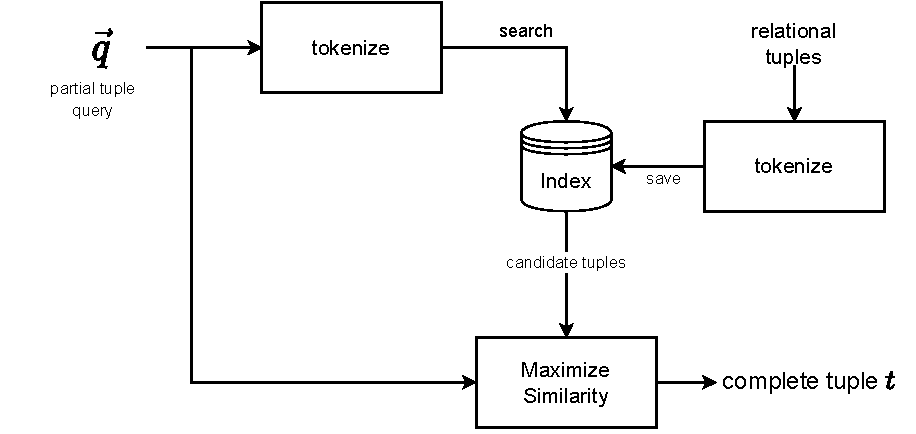
\includegraphics[width=0.8\textwidth]{my/graphics/tuple_completion.pdf}
	\caption{Matching a partial tuple $\vec{q}$ to a complete tuple $t$}
	\label{fig:tuple_completion}
\end{figure}

We use a neural network to optimize the query processing pipeline. Detailed description can be found in  Section~\ref{sec:opt_pipeline}. We define the neural network classifier as:

\begin{definition}[Neural network classifier]
%	what is the input to the neural network, and what you are learning?
	Let $R_1, R_2, R_3, \dots, R_K$ be $K$ relations. The neural network classifier takes a partial tuple query $\vec q$ and estimates the probabilities that the search result of $\vec q$ belongs to relation $R_i$, $\forall i \in \{1, 2, \dots, K\}$.
	%Let $\mathbf{index}_1$, $\mathbf{index}_2$, $\dots$, $\mathbf{index}_K$ be $K$ full-text indexes corresponding to the $K$ relations.

 
%	Given a set of $N$ training examples $\mathbb X = \{(x^{(i)}, l^{(i)}): i = 1, 2, \dots, N\}$, where  $x^{(i)}$ is a (partial) tuple that belongs to $R_{l^{(i)}}$ ($l^{(i)} \in \{1, 2, ..., K\}$),
%	the goal is to train a neural network classifier that takes a partial tuple query $\vec q$ and estimates the probabilities that the search result of $\vec q$ belongs to relation $R_i$, $\forall i \in \{1, 2, \dots, K\}$.
\end{definition}

%	Note that we use full-text index to support partial tuple search, and we partition full-text index to mitigate the impact of bottleneck casued by hashing collision in inverted term index data structure. More details about partitioning of full-text index are given in Section~\ref{subsection:partition_text_index}.

\section{Partial tuple search using full-text search}
\label{sec:search_fulltext_index}
Traditional full-text indexes, such as Apache Lucene, support keyword queries over large document collections using an inverted index data structure.  In this section, we describe how a full-text index is incorporated as the first stage of the query processing pipeline for partial tuple search.

The advantages of using a full-text index are:

\begin{itemize}
    \item Flexible and partial string matching between query keywords and document text
    \item Efficient query processing provided that the inverted document lists are not too long due to collisions.
\end{itemize}

We first encode complete relational tuples as documents to be stored in the full-text index.
The partial tuple query $\vec q$ is encoded as a keyword query.  It is important to point out that we must specify
the same tokenizer to convert relational tuples and query tuples to tokenized terms.  We use the 3-gram tokenizer to support fuzzy string matching for the values.

The full-text index evaluates the keyword query, and computes a top-$k$ result set of the best matching documents as relational tuple candidates.  These top-$k$ candidates guarantee high similarity between the labeled values in $\vec q$ and those in relational tuples.

\subsection{Encoding of tuples as documents}

Let us denote the tokenizer function as $\Tokenize$. A tuple $\vec r$ is converted into a document $\mathrm{doc}$ as follows:

$$
\Attr(\mathrm{doc}) = \Attr(\vec r) \cup \{\mathtt{fulltext}\}
$$
For each $a\in\Attr(\vec r)$,
$$
\mathrm{doc}[a] = \Tokenize(\vec r[a])
$$
Also,
$$
\mathrm{doc}[\mathtt{fulltext}] =\bigcup\big\{\Tokenize(\vec r[a]): a\in\Attr(\vec r)\big\}
$$
The special field $\mathtt{fulltext}$ of $\mathrm{doc}$ contains all tokenized terms of the tuple $\vec r$.

\begin{example}
Given a tuple $\vec r$ as:
$$
(\mathrm{Name}:Jack,\ \mathrm{Address}:100\ Simcoe\ Street)
$$
Its attributes $\Attr(\vec r)$ are $\{\mathrm{Name}, \mathrm{Address}\}$. Therefore, the document attributes  $\Attr(doc)$ are $\{\mathrm{Name},\ \mathrm{Address},\ \mathrm{fulltext}\}$.

If we use a standard tokenizer, the result of tokenization will be,
$$
\left[\begin{array}{rcl}
\mathrm{Name} & \mapsto & \makebox{Jack} \\
\mathrm{Address} & \mapsto & \makebox{100, Simcoe, Street} \\
\mathrm{fulltext} & \mapsto & \makebox{Jack, 100, Simcoe, Street}
\end{array}\right]
$$

On the other hand, if we use a character-based 3-gram tokenizer with a special padding character ``\_", the result will be,
$$
\left[\begin{array}{rcl}
\mathrm{Name} & \mapsto & \makebox{\_\_J \_Ja Jac ack ck\_ k\_\_} \\
\mathrm{Address} & \mapsto & \makebox{\_\_1 \_10 100 00\_ 0\_\_ \_\_S \_Si Sim imc mco coe oe\_ e\_\_ \_\_S \_St Str tre ree eet et\_ t\_\_} \\
\mathrm{fulltext} & \mapsto & \makebox{\_\_J \_Ja Jac ack ck\_ k\_\_ \_\_1 \_10 100 00\_ 0\_\_ \_\_S \_Si Sim imc mco coe oe\_ e\_\_ \_\_S} \\ 
 & & \makebox{\_St Str tre ree eet et\_ t\_\_}\\
\end{array}\right]
$$

\end{example}

\subsection{Encoding partial tuple queries as keyword queries}

Given a partial tuple $\vec q$, we want to encode it as a keyword query such that the search engine can
find the documents that correspond to the relevant tuples.

For each labeled value $(l_i, x_i)$ in the partial tuple, we generate a query clause.

\begin{itemize}
\item If $l_i\not= ?$, then the query clause is $q_i = l_i:x_i$.
\item If $l_i = ?$, then the query clause is $q_i = \mathtt{fulltext}:x_i$.
\end{itemize}

The generated query is:
$$ q = q_1\ \mathbf{or}\ q_2\ \mathbf{or}\ \dots $$

One can see that any complete tuple $\vec r$ that satisfy the query $\vec q$ will have its encoding document satisfying the keyword query $q$.

\subsection{From search results to partial tuple completion}

For our problem, we need to match the partial tuple $\vec q$ with a complete tuple $t$.  This can be done
by further post-process the documents in search results returned by the search engine. 

%Recall that a tuple matching is a function $h: \mathrm{LV}(t) \to \mathrm{LV}(\vec q)$.  
Recall that a tuple matching is a function $h: \mathrm{LV}(\vec q) \to \mathrm{LV}(t)$, where $\mathrm{LV}(\vec q)$ and $\mathrm{LV}(t)$ are labeled values of $\vec q$ and $t$, respectively.
The top completion of $\vec q$ should be a complete tuple that has the highest matching score based on the similarity measure.  Since the search engine already returns the top-$k$ candidate documents, we can compute the optimal matching
between $\vec q$ to each of the candidates in order to rank the candidates with respect to their matching scores.

Finding optimal matching of labeled values from the partial tuple $\vec q$ to  a candidate tuple $t$ is equivalent to solving the maximum weighted matching of a bipartite graph.

Define the graph $G$ as:
\begin{itemize}
    \item The vertices are: $V = \mathrm{LV}(t)\cup\mathrm{LV}(\vec q)$.
    \item The edges and their respective weights are defined as:
        $$E = \{\left<x_1, x_2, \Sim(V(x_1),V(x_2)\right>: x_1\in\mathrm{LV}(t)\makebox{ and }
        x_2\in\mathrm{LV}(\vec q)
        \makebox{ and } (L(x_1)=L(x_2) \makebox{ or } L(x_2)=?)\}$$ 
       where $L(x_1)$ and $L(x_2)$ are labels of $x_1$ and $x_2$, respectively.
    \item $G$ is the weighted graph $(V, E)$.
\end{itemize}

%The max-weighted matching of $G$ is necessarily a matching $h$ from $\mathrm{LV}(t)$ to $\mathrm{LV}(\vec q)$.
The max-weighted matching of $G$ is necessarily a matching $h$ from $\mathrm{LV}(\vec q)$ to $\mathrm{LV}(t)$.
The weight sum of $h$ is the matching score based on the similarity of matched labeled values.  It is now that the optimal matching can be
found exactly in polynomial time using various algorithms, e.g., Hungarian algorithm \cite{cormen2022introduction}.



\section{Optimizing query processing pipeline with neural networks}
\label{sec:opt_pipeline}

As described in Section~\ref{sec:fuzzy-collision}, a potential bottleneck associated with inverted index structures for full-text search is the hashing collision which creates long linked lists
at the leaf nodes of the index tree (See Figure~\ref{fig:inverted_term_index}).

In our application, the character based 3-gram tokenizer will generate a compact vocabulary consisting
of at most $|\mathrm{charset}|^3$ distinct tokens where $\mathrm{charset}$ is the total character set.  So, when the number of documents grow greater than $|\mathrm{charset}|^3$, the linked lists at the leaf nodes will grow linearly with respect to the number of relational tuples.

The concern is that the full-text index will degrade as the dataset size grows due to the 3-gram tokenization that we employ to support fuzzy string matching.  Unfortunately, our experimental evaluation in Section~\ref{subsection:perf_baseline_expt} confirms the performance degradation in practice.

In this section, we will describe a method to perform partitioning of the full-text index to overcome the performance bottleneck caused by hash collisions.

Our method utilizes a neural network to optimize the index access order during partial tuple search.  The neural network is to be embedded in the overall query processing pipeline, and will be self-supervised based on existing data.

\subsection{Partition of full-text index}
\label{subsection:partition_text_index}
An aggregated index is a function as follows:
$$\mathbf{index} : \mathbf{Query} \to \mathbf{List}[\mathbf{Tuple}]$$
It indexes all the tuples from every relation.

However, we advocate to partition the tuples based on the relation they below to.  Thus,
if we have relations $R_1, R_2, R_3, \dots, R_n$, we will have $n$ indexes
$\{\mathbf{index}_1$, $\mathbf{index}_2$, $\dots$, $\mathbf{index}_n\}$, each indexing the tuples
of a single relation.

$$\mathbf{index}_i : \mathbf{Query} \to \mathbf{List}[\mathbf{Tuple}]$$

The search can be done concurrently over all indexes:

\begin{verbatim}
priority_queue
for index_i in all_indexes {
  spawn index_i.search(q) into priority_queue
}
\end{verbatim}

We can also do sequential access of the indexes:

\begin{verbatim}
for index_i in sorted(all_indexes, q) {
    index_i.search(q) into priority_queue
}
\end{verbatim}

In this thesis we focus on the sequential access approach in favour of saving CPU load.
The challenge is to sort the indexes dynamically based on the user query $\vec q$.
The sorting should place relations that can satisfy $\vec q$ with higher priority, so that
successful matches are found as early as possible.

Thus, our strategy to sort the indexes is based on a sorting key function:
$$
S : (\mathbf{index}_i, \vec q) \to [0, 1] \mapsto \mathbf{prob}(\mathrm{result}(\vec q) \in R_i)
$$

The sorting score $S(\mathbf{index}_i, \vec q)$ is the (estimate of the) probability that the search
result of $\vec q$ belongs to the relation $R_i$.  Since there are only a finite many relations,
we can reformulate the scoring function $S$ to as an $n$-way classification function:

$$
\mathbf{classify} : \vec q \mapsto \left[
\begin{array}{c}
    S(\mathbf{index}_1, \vec q) \\
    S(\mathbf{index}_2, \vec q) \\
    \vdots \\
    S(\mathbf{index}_n, \vec q)
\end{array}
\right]
$$

Our objective is to learn the $\mathbf{classify}$ function using a neural network.

\subsection{Vectorization of queries}

The classifier can be trained using a neural network that can be embedded in the query processing pipeline.
The design objectives are:
\begin{itemize}
    \item The neural network must be compact in size so that it incurs minimal performance overhead, and can be embedded in a search system.
    \item The training of the network must require minimal manual intervention.  Thus the neural network must be trained with self-supervision from existing data.
\end{itemize}

The classification function is:

\begin{equation}
    \mathbf{classify} : \mathbf{Query} \to \mathbb{R}^n
\end{equation}
where the output of $\mathbf{classify}$ is the probability distribution over the $n$ partitioned indexes. Elements we presented in Section~\ref{sec:neural-networks} present several options for the neural network architecture.

\noindent{\bf Token representation of queries}:  given a query $\vec q=\{(l_i, x_i): 1\leq i \leq m\}$, we generate the text representation of the query by simply concatenating the text representation of labels and the tokenized query values.

$$
\mathbf{tokens}(\vec q) = \{l_1\} \oplus \mathbf{tokenize}(x_1) \oplus \{l_2\} \oplus \mathbf{tokenize}(x_2) \oplus \dots
\{l_m\} \cup \mathbf{tokenize}(x_m)
$$
where $\oplus$ is sequence concatenation.

\noindent{\bf Integer encoding of queries}: next we encode $\mathbf{tokens}(\vec q)$ using a universal
vocabulary $\mathbf{vocab}$.  The vocabulary consists of all known tokens, and their respective
ordinal integer code.  This vocabulary will be built using the existing relational tuples.  The construction of the vocabulary is described in subsequent sections.  The vocabulary is described as a function from tokens to integers:
$$ \mathbf{vocab} : \mathbf{Token} \to \mathbb{N}$$

The integer sequence of a query is given by:
$$
\mathbf{sequence}(\vec q) = \mathbf{vocab}\circ\mathbf{tokens} (\vec q) \in\mathbb{N}^*
$$

\noindent{\bf Embedding vectors of queries}:
Using a standard embedding layer (Section~\ref{sec:embedding-layer}), embed the integer sequence representation of the query
to a sequence of latent vectors.

$$
\mathbf{vector}(\vec q) = \mathbf{Embedding}(\mathbf{sequence}(\vec q))\in\mathbb{R}^{|q|\times d}
$$

At this point, we have many options in mapping
the vector sequence to the probability distribution
in $\mathbb{R}^n$.

For the remainder of this chapter, we denote the vector sequence representation of $\vec q$ as:

$$\vec x = \mathbf{sequence}(\vec q) = (x_1, x_2, \dots, x_{|q|})$$
where each $x_i\in\mathbb{R}^d$ is the embedding vector 
of the $i$-th token in a $d$-dimensional latent space.

\subsection{Neural network architectures for query classification}
\label{sec:architectures}

\noindent{\bf MLP based classification}.

Given the input of vectorized query representation $\vec x$, 
we first flatten it using global average over the entire sequence length.  Then, we process it with a MLP with softmax
activation function.  The MLP must have $n$ output neurons.

$$
\begin{array}{rlr}
&\vec x  & (|q|, d) \\
\to & \left(\frac{\sum_{i=1}^{|q|} x_i}{|q|}\right) & (d) \\
\to & \mathbf{MLP}(\makebox{output-dim}=n) & (n) \\
\to & \mathbf{softmax}(\cdot) & (n) \\
\end{array}
$$

\noindent{\bf Recurrent network architecture with LSTM cells}.

Since recurrent neural networks (RNN) are specifically designed to process sequence inputs, we can utilize
a RNN to map the input $\vec x$ to a flattened state vector, which can then be processed
by a MLP to compute the output probability distribution.

The advantage of RNN is that it can learn inter-token dependencies in the query at the cost of
a bigger model size and higher training cost.

$$
\begin{array}{rlr}
&\vec x  & (|q|, d) \\
\to & \mathbf{LSTM}(\makebox{output-state=True}) & (d) \\
\to & \mathbf{MLP}(\makebox{output-dim}=n) & (n) \\
\to & \mathbf{softmax}(\cdot) & (n) \\
\end{array}
$$

\noindent{\bf 1D convolution architecture}.

Another standard technique to learn sequential features is to use 1D convolution.
The 1D convolution layer (Section~\ref{sec:cnn}) produces a sequence of {\em feature} vectors
that capture the short-range token dependencies within the convolution window size.  We then use
global averaging to flatten the convolution features for further processing using a MLP.

$$
\begin{array}{rlr}
&\vec x  & (|q|, d) \\
\to & \mathbf{Conv1D} & (|q|, d) \\
\to & \mathbf{Global\ Average} & (d)\\
\to & \mathbf{MLP}(\makebox{output-dim}=n) & (n) \\
\to & \mathbf{softmax}(\cdot) & (n) \\
\end{array}
$$

\noindent{\bf Transformer and MLP Mixer}

Transformers have shown to be a superior architecture for many tasks in the domain of MLP and sequence learning.  The exact architecture of a transformer block is shown in the implementation section (See Figure~\ref{fig:transformer_model}).  Due to the nature of our problem, we chose to use only a single transformer block so that the model remains small enough to be embedded in the query processing pipeline.

A more recent MLP based architecture is MLP mixer which is a concatenation of two MLP layers separated by a matrix transpose operation.  Details of the MLP mixer are shown in Figure~\ref{fig:mlpmixer_model}.

\subsection{Unsupervised training of neural network classifiers}

The classifier needs to be trained with data of the following form:
$$
(\vec q, i)
$$
where $\vec q$ is a sample query, and $i$ is the relation $R_i$ that contains the best matching
tuple of $\vec q$.

The training data is generated directly from the relational tuples from the database.  For each complete tuple $\vec r = \{(l_i, x_i): i\in I\}$, we formed a query $\vec q_r$ by random sampling from
the labeled values while masking the labels.

$$
\vec q_r = \{(?, x_i): i\in\mathbf{sample}(I)\}
$$

Thus, given a database with $n$ relations $R_1, R_2, \dots, R_n$:
$$
\mathbf{train} = \bigcup_{i=1}^n\{(\vec q_r, i): r\in R_i\}
$$

\section{Overall query processing pipeline}

To summarize the proposed query processing pipeline for partial tuple search, we have the following stages:

\begin{enumerate}
    \item A partial tuple is entered as user input.
    \item The partial tuple is tokenized and converted to a structured keyword query.
    \item The neural network classifier sorts the partitioned indexes based on the probability scores.
    \item The partitioned indexes are scanned to find top-$k$ complete tuple candidates from the database.
    \item The candidates are ranked by max-matching based similarity scores.
\end{enumerate}

Our pipeline requires that partitioned full-text indexes are built from tuples of each relation in offline mode. In addition, the neural network classifier should be trained using sampled tuples from each relation.

In Chapter~\ref{ch:implementation-evaluation}, we will describe the implementation of each neural network architecture. We will also discuss the experimental evaluation and comparison of the performance gain of each neural network architecture.